\section{Experimental Reach}

The primary search channel for this experiment is, $A' \rightarrow e^+ e^-$, with or without
 a displaced vertex, depending on the magnitude of the coupling $\alpha'$. As such, 
the primary irreducible 
background is QED trident production, with rate given by the diagrams shown in 
Figure \ref{fig:apdiagram}. Trident events can be usefully separated into ``radiative'' diagrams 
(Figure \ref{fig:radbhdiagram}(a)), and ``Bethe-Heitler'' diagrams (Figure \ref{fig:radbhdiagram}(b)), that are separately 
gauge-invariant.  The expected parameter reach of the experiment is shown in Figure \ref{fig:reach}.  Below, we discuss how this was calculated.  

The contribution from the radiative diagrams (Figure \ref{fig:radbhdiagram}(a)) alone is a useful guide 
to the behavior of A' signals at various masses.  In particular, the kinematics of A' 
signal events is identical to that of radiative trident events restricted to an invariant 
mass window near the A' mass.  Moreover, the rate of the A' signal is simply related to 
the radiative trident cross-section within a small mass window of width $\delta m_{A'}$  
by [1],
\begin{equation}
 {{d\sigma(e^-Z\rightarrow e^-Z(A'\rightarrow e^+e^-))} \over
    {d\sigma(e^-Z\rightarrow e^-Z(\gamma^*\rightarrow e^+e^-))}} =
    ({{3\pi \epsilon^2} \over {2N_{eff}\alpha}}) ({{m_{A'}} \over {\delta m_{A'}}})
  \label{eqn:radToAprime}
\end{equation}
where $N_{eff}$ counts the number of available decay states.  A fraction $\epsilon_{bin}$ 
of signal events will have reconstructed masses within the mass window, because of the 
finite mass resolution  (for a $2.5 \times \sigma$ mass resolution window, 
$\epsilon_{bin}$= 0.8).  Equation \ref{eqn:radToAprime} corrected for $\epsilon_{bin}$ allows us to 
conveniently express the sensitivity to A' signals in terms of the radiative portion 
of the total QED trident statistics, which we will do shortly. 

The Bethe-Heitler process has a much larger total cross-section than either the signal 
or the radiative trident backgrounds, but exploiting its different kinematics can 
significantly reduce it. In particular, the A' carries most of the beam energy 
(see the discussion in Section \ref{sec:apsignal}) while the recoiling electron is very soft and 
scatters to a wide angle. In contrast, the Bethe-Heitler process is not enhanced at 
high pair energy. Moreover, Bethe-Heitler processes have a forward singularity that 
strongly favors asymmetric configurations with one energetic, forward electron or 
positron and the other constituent of the pair much softer.   The geometric acceptance and trigger 
requirements select the region of phase space where signal is dominated, and the 
Bethe-Heitler background is smallest, as illustrated by Figure \ref{fig:tridentkinematics} (it should be 
emphasized, however, that even in this region the Bethe-Heitler background rate exceeds 
that of radiative tridents by roughly a factor of 5).  The radiative and Bethe-Heitler  cross-sections, after accounting for acceptance
in the HPS detector, are shown in Figure \ref{fig:bkgXS}.

\begin{figure}
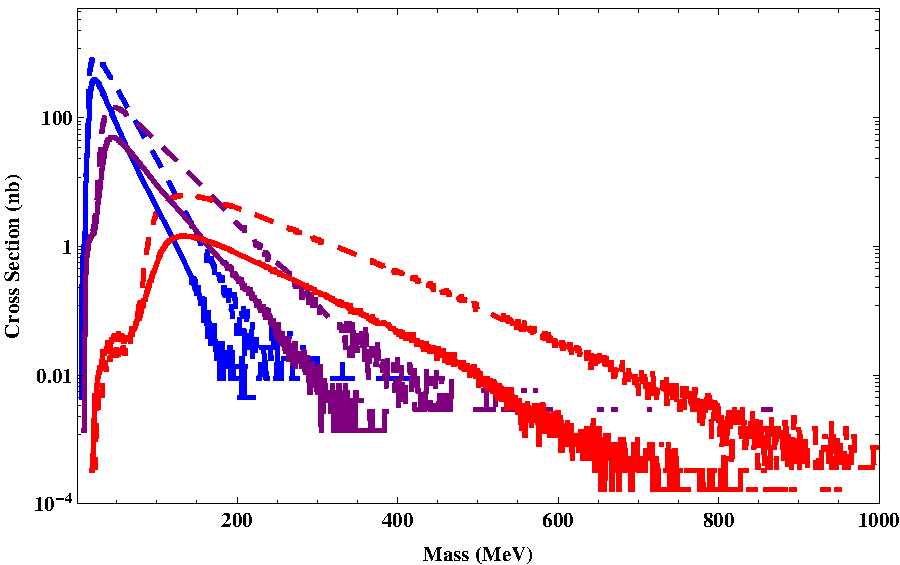
\includegraphics[scale=1]{reach/HPS-CrossSections.pdf}
\caption{The Bethe-Heilter (dashed) and radiative (solid) cross-section/MeV after acceptance for 1.1 (blue), 2.2 (purple) and 6.6 GeV (red).}
\label{fig:bkgXS}
\end{figure} 

To compute the reach of the HPS experiment, we simulate the production of irreducible 
trident reactions in the detector. We additionally apply a mock-up of the geometric 
acceptance for the tracking and of the trigger requirements.  In addition, high-statistics 
Monte Carlo samples at particular invariant masses have been used to estimate 
the background rejection efficiency for a vertex-based search.  
We produce generator-level events using MadGraph and MadEvent \cite{Alwall:2007st}  to compute the full 
matrix elements for $e^-Z \rightarrow e^- (e^+ e^-)Z$ in leading order QED, but 
neglecting the effect of nuclear excitations on the kinematics in inelastic processes. 
We use the QED nuclear elastic and inelastic electric form-factors in\cite{Kim:1973he}. The MadEvent 
code was modified to properly account for the masses of the incoming nucleus and electron 
in event kinematics.

We use a ``reduced-interference'' approximation that simplifies our analysis and is much 
less computationally intensive.  In this approximation, we treat the recoiling $e^-$ and 
the $e^-$ from the produced pair as distinguishable. Furthermore, we separate trident 
processes into the radiative diagrams and the Bethe-Heitler diagrams, and
 we calculate the cross-section for both of these diagrams separately.
 Within the acceptance and signal region for the HPS experiment, the Bethe-Heitler 
reactions dominate the trident rate by 4:1. We have checked that the ``reduced-interference''
 approximation does not correct the trident cross-section by more than 10\% in a 
representative kinematic region [4].



\subsection{Resonance Search}


\begin{figure}
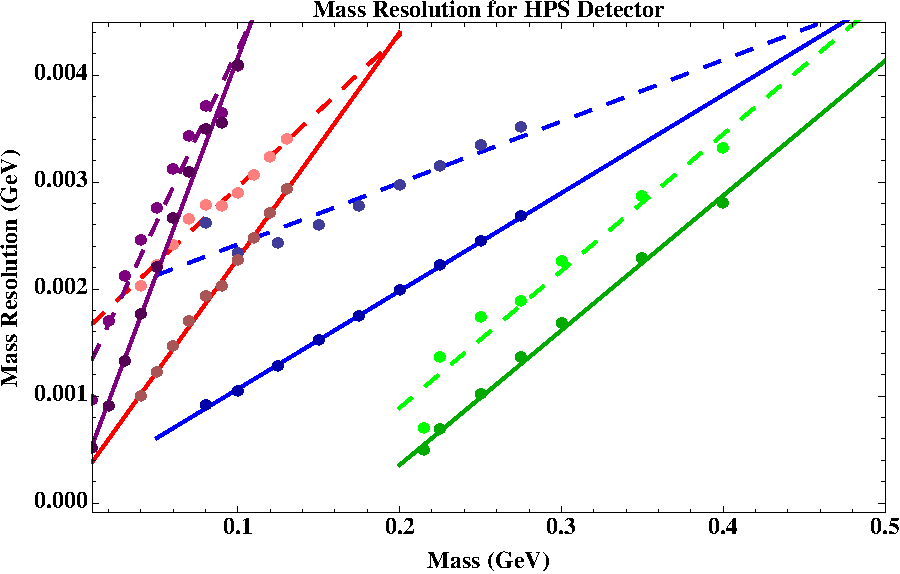
\includegraphics[scale=1.0]{reach/mass-resolution.pdf}
\caption{The invariant mass resolution versus mass for 1.1 (purple), 2.2 (red), 6.6 GeV  electron decays  (blue) and 6.6 GeV muon decays (green).  
The points are from simulated data at various masses while the lines are linear fits to the points.  For each energy, the points with worse resolution (dashed line) are from the vertex fit without constraining the decay to the target while the better resolution (solid line) require the decay to be prompt.
The fitted curves are used in the reach calculation; the resolution from the dashed lines are used for the displaced vertex search while the bump-hunt search uses the resolution from the solid lines.}
\label{fig:massresReach}
\end{figure} 

\begin{figure}
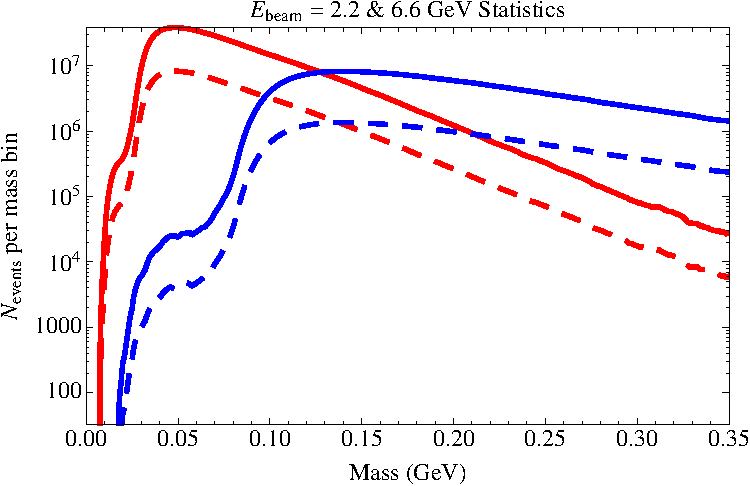
\includegraphics[scale=1.0]{reach/TotalStats.pdf}
\caption{Right: Distribution of statistics in full resonance search.
  The solid (dashed) curves indicate the number of background QED trident (radiative) events expected in a 
  resolution-limited mass window of width $\delta m_(A' )=2.5 \sigma (m_{A'})$.  The red 
curve corresponds to the distribution of statistics for a one month run at 6.6 GeV 
beam energy (blue), with a current of 450 nA on a 0.25\% $X_0$ target, while the dashed maroon 
curve corresponds to six weeks  at 2.2 GeV beam energy (red) and a 0.125\% $X_0$ target.}
\label{fig:totalStats}
\end{figure} 
%
%Figure 6.1.1.   Right: Distribution of statistics in full resonance search.
%  The curves indicate the number of background QED trident events expected in a 
%resolution-limited mass window of width $\delta m_(A' )=2.5 \sigma (m_{A'})$.  The red 
%curve corresponds to the distribution of statistics for a one month run at 6.6 GeV 
%beam energy, with a current of 450 nA on a 0.25\% $X_0$ target, while the dashed maroon 
%curve corresponds to six weeks  at 2.2 GeV beam energy and a 0.125\% $X_0$ target.

Equation \ref{eqn:radToAprime} is used to compute the reach for a resonance search in the $e^+ e^-$ or 
$\mu^+ \mu^-$ final state. We start by simulating radiative and Bethe-Heitler trident 
events and require that $e^+ e^-$ or $\mu^+ \mu^-$ pairs pass the detector acceptance cuts. 
We additionally require that the total energy exceed 80\% or the beam energy and that each 
track have at least 0.5 GeV of energy. We will refer to these cuts collectively as the 
``detector/trigger mock-up''. We compute the total differential cross section, as 
a function of invariant mass, for radiative and Bethe-Heitler trident events to pass the 
detector/trigger mock-up cuts, and from this the final statistics is computed assuming 
a run duration according to the run plan laid out in Section \ref{sec:measurements}, and conditions in Section \ref{sec:trkperf}.
The  mass resolution  and the background statistics expected in each resolution-limited mass window are shown 
in Figures \ref{fig:massresReach} and \ref{fig:totalStats}.


To quantify statistical sensitivity, we assume that the trident background in the 
resonance search can be modeled by a smoothly varying function and subtracted off. 
The significance is then determined by the ratio of the signal within an invariant mass 
window to $\sqrt{N_{bin}}$, where $N_{bin}$ is the total background statistics in the 
same window. Using equation \ref{eqn:radToAprime}, the sensitivity for a resonance search is determined by
\begin{equation}
 \left({{S} \over {\sqrt{B}}}\right)_{bin}=\left({{N_{radiative}} \over {N_{total}}}\right) \sqrt{N_{bin}} 
\left({{3\pi \epsilon^2} \over {2 N_{eff}\alpha}}\right)\left({{m_{A'}} \over {\delta m_{A'}}}\right)
\epsilon_{bin}
\label{eqn:signifBumpHunt}
\end{equation}   
Here, $({{N_{radiative}} \over {N_{total}}})$ is the fraction of radiative reactions 
among all QED trident events in the search region. This quantity is determined by 
simulation as described below. $N_{bin}$ is the total number of QED trident events 
residing in a given invariant mass search bin, and is determined by
\begin{equation}
 N_{bin} \equiv \epsilon_{reco}^2 \times \epsilon_{stat}(m_{A'})
 \times \sigma_{trigger} \times L.
\end{equation}
Here $L$ is the integrated luminosity, $\sigma_{trigger}$ is the trigger cross section, 
$\epsilon_{stat} (m_{A'})$ is the fraction of the total statistics in an invariant 
mass window centered on $m_{A'}$ of size  $\delta m_{A'} =2.5 \sigma (m_{A'})$, 
and $\epsilon_{reco} \cong 0.85$ is the efficiency for reconstructing each track that is 
within the geometric acceptance of the detector. 

\subsection{ Displaced Vertex and Resonance Search}

A search for resonances that decay with cm-scale displaced vertices opens up sensitivity 
to much smaller couplings than can be observed through a resonance search alone.  
The vertex reconstruction and quality selection is discussed in Section \ref{sec:trkperf}.   
For the purpose of computing reach, the vertex quality requirements 
reduce the signal efficiency by a factor  $\sigma_{sig}\sim 0.5$.  
We use the high-statistics Monte Carlo studies described in 
Section \ref{sec:trkperf} to model the tails of the vertex distribution for decays at the target.  
These vertex distributions have been generated at a few different masses for each beam energy. 
Away from  these masses, we parameterize the background rejection factor $\epsilon_{rejection} (zcut)$,
 the fraction of events with a fake vertex beyond a beam line distance of zcut, 
by a smooth interpolation.

%In Figure \ref{fig:tracking distribution}, we show the distribution of fake vertices in the z-direction along 
%the beam line, as well as the distributions for signals corresponding to 
%${{\alpha'} \over {\alpha}}=10^{-8.5}$ and $10^{-9.5}$, as well as for true muonium (see Section \ref{}).

%make this plot again?  

%Figure 6.2.1 Signal and background vertex distributions in a resolution-limited invariant 
%mass window, over the $3 \times 10^6$s run period at 5.5 GeV (note the different run conditions).  
%The black curve represents the fake vertex distribution from trident events with mass in a 
%$2.5\sigma (m_{A'})$ window about 200 MeV.  The red and yellow curves are the vertex distributions 
%for signal events from an A' of the same mass, with $\alpha ' / \alpha$ = $10^{-8.5}$ ($\gamma c\tau $
%=3.5 mm) and $\alpha ' /\alpha$ =$10^{-9.5}$ ($\gamma c\tau$=35 mm), respectively.  The blue curve 
%corresponds to the rate and vertex distribution expected from l=1 (triplet) state of true muonium, 
%with $\gamma c\tau$=14.2 mm (see Section 6.4).

Because the fake vertex distribution falls quite rapidly, the greatest sensitivity is achieved far 
on the vertex tail, where less than one background event is expected.  For the purpose of 
computing reach, we have determined a mass-dependent choice of $zcut(m_{A'})$ such that the 
expected background in each resolution-limited mass window $\delta m_{A'}$, with reconstructed 
vertices beyond this cut, does not exceed 0.5 events in the run period.  
This requires rejection $\epsilon_{rejection} (zcut)$ of background events from the target at 
the level of $10^{-6}$ to $10^{-7}$, achieved for $zcut \sim$5-30 mm (see Figure \ref{fig:vtxLength}). 


\begin{figure}
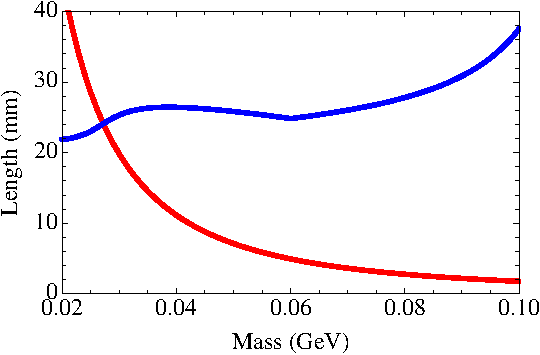
\includegraphics[scale=0.8]{reach/decay-lengths-2pt2.pdf}
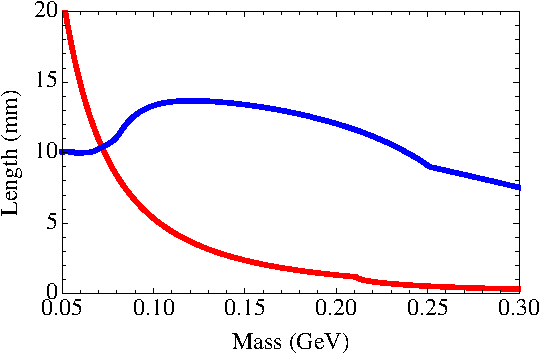
\includegraphics[scale=0.8]{reach/decay-lengths-6pt6.pdf}
\caption{In blue:  the minimum vertex displacement $z_{min}$ (in mm) along the beamline, required for 
the vertex-based resonance search at 2.2 GeV (left) and 6.6 GeV (right).  These are chosen 
to bring the expected background to 0.5 events in each resolution-limited mass window. 
 In red:  the $\gamma c\tau$ assuming $\epsilon=10^{-4}$.}
\label{fig:vtxLength}
\end{figure} 


 The geometric acceptance falls off at  decay lengths greater than 10 cm.  
For simplicity we compute reach using the geometric acceptance for z=0, but only considering 
decays with $z<zmax$=10 cm, so that the fraction of signal events included in the vertex search is
\begin{equation}
\epsilon_{sig} (zcut) \cong \epsilon_{vtx} \times\left (e^{-{{zcut} \over {\gamma c\tau}}} - e^{-{{zmax} \over {\gamma c\tau}}}\right).
\end{equation}

Accounting for the reduced acceptance of both signal and background events, the statistical 
significance expected for a given value of can be computed from that of the pure resonance 
search as  an expected signal can be computed by

\begin{equation}
 \left({{S} \over {\sqrt{B}}}\right)_{bin,zcut}=\left ({{S} \over {\sqrt{B}}}\right)_{bin}  
{{\epsilon_{sig} (zcut)} \over {\sqrt{\epsilon_{rejection} (zcut)}}} >2
\label{eqn:signifVertex}
\end{equation}
where $({{S} \over {\sqrt{B}}})_{bin}$ is given by \eqref{eqn:signifBumpHunt}. For the small expected background rate 
(0.5 events/bin), however, this formula becomes irrelevant, as the exclusion sensitivity of 
the experiment is limited by the probability of a downward fluctuation in the signal.  
Thus, for the vertex reach contours in Figure \ref{fig:reach}, we additionally require 
an expected signal
\begin{equation}
 S_{bin,zcut}=\left({{N_{radiative} \over {N_{total}}}}\right) N_{bin} 
\left({{3\pi \epsilon^2} \over {2 N_{eff}\alpha}}\right) \left({{m_{A'}} \over {\delta m_{A'}}}\right) \epsilon_{sig}
 (zcut) > 2.4~ {\rm events} 
 \label{eqn:signalVertex}
\end{equation}

\subsection{Reach in Mass-Coupling Parameter Space}

Using the $S/\sqrt(B))$ for the bump-hunt  and displaced vertex searches as described above, we estimate to cover the regions of coupling vs mass parameter space shown in Figure \ref{fig:reachDetailed}.  The contours in the plot show the the two-sigma exclusion regions for:
\begin{itemize}
\item purple, dashed: 1 week of 50nA, 1.1 GeV beam on a 0.125\% target
\item blue, dashed: 1 week of 200nA, 2.2 GeV beam on a 0.125\% target
\item blue, solid: 3 weeks of 200nA, 2.2 GeV beam on a 0.125\% target
\item dark green: 2 weeks of 450nA, 6.6 GeV beam on a 0.25\% target, detecting $A^\prime\rarr e^+e^-$
\item light green: 2 weeks of 450nA, 6.6 GeV beam on a 0.25\% target, detecting $A^\prime\rarr \mu^+\mu^-$
\item red:  the statistical combination of all of the above
\item green shaded:  3 months each of 2.2 GeV and 6.6 GeV (same currents and thicknesses as above)
\end{itemize}



\begin{figure}
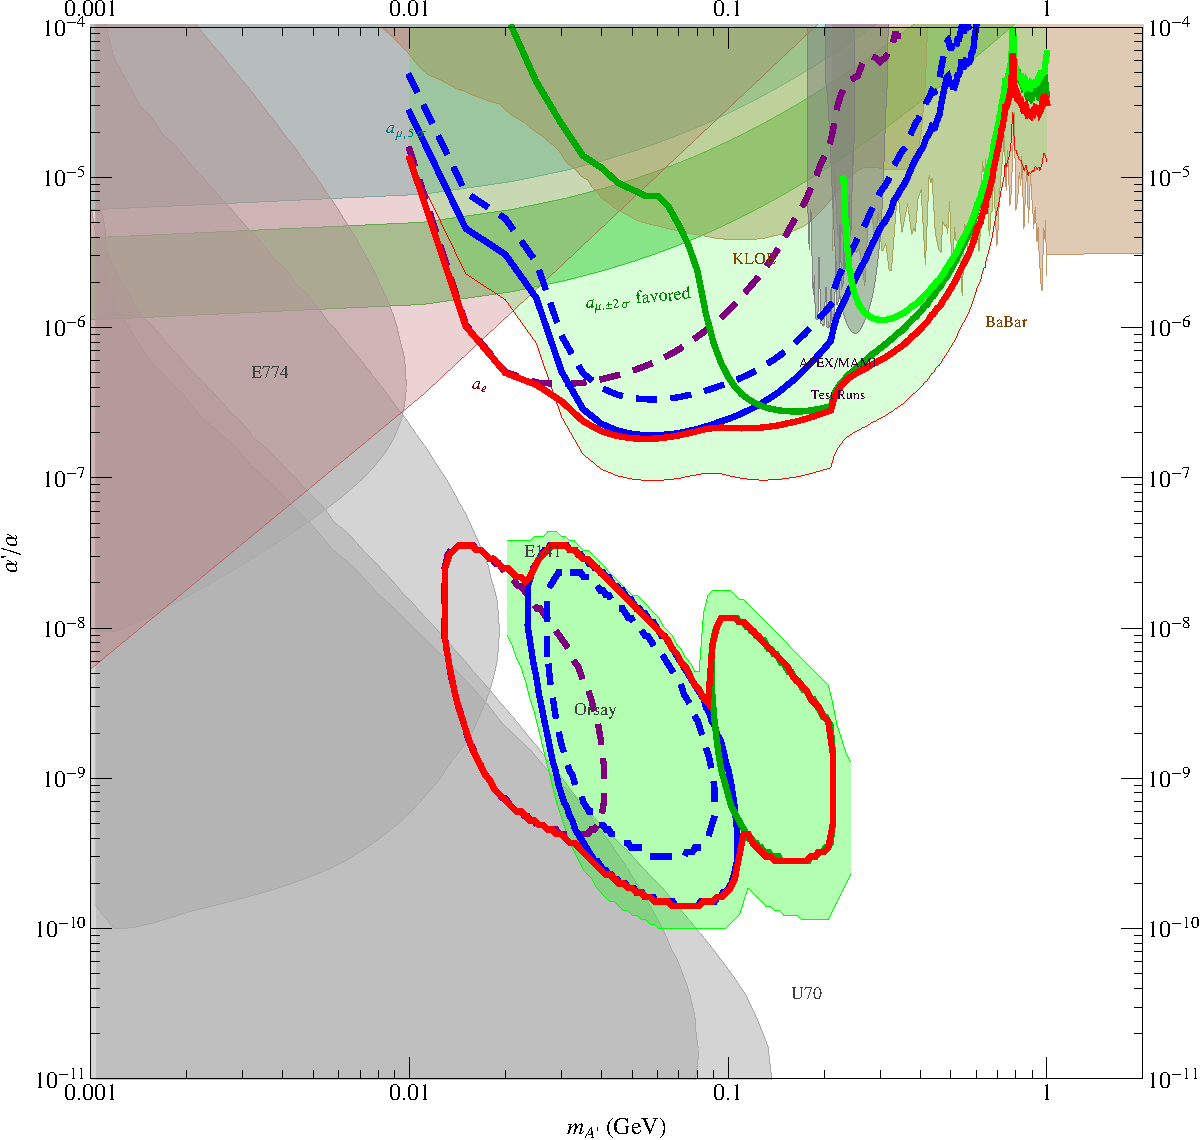
\includegraphics[scale=0.8]{reach/HPS-Proposal2014-DetailedReach.pdf}
\caption{The expect reach in mass-coupling parameter space.  See text for details about different features.}
\label{fig:reachDetailed}
\end{figure} 



